\documentclass[border=0.8ex,svgnames,tikz]{standalone}
\usepackage{amsmath,mathtools}
\usepackage{fontspec}
\setmainfont{Source Serif 4}
\setsansfont{Source Sans 3}
\setmonofont{Source Code Pro}

\usetikzlibrary{positioning,calc}

\begin{document}
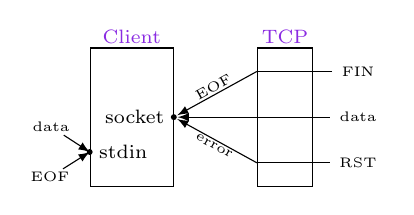
\begin{tikzpicture}
  % client
  \begin{scope}[
    every node/.append style={inner sep=0.75ex,font=\scriptsize},
    every edge/.style={draw,fill=none,>=latex},
    input node/.style={font=\tiny,inner sep=0.25ex},
    ]
    \node[draw,minimum width=3em,minimum height=5em] (client) at (0,0) {};
    \coordinate(socket-input) at (client.east);
    \coordinate(stdin-input) at ($(client.west)!0.5!(client.south west)$);
    \node[input node,above left=2ex of stdin-input] (stdin-data) {data};
    \node[input node,below left=2ex of stdin-input] (stdin-eof)  {EOF};
    \node[circle,inner sep=0.2ex] (socket-node) at (socket-input) {};
    \path[fill=Black]
    (stdin-input) circle (0.25ex) node[right]{stdin}
    (socket-input) circle (0.25ex) node[left]{socket}
    (stdin-data) edge[->] (stdin-input)
    (stdin-eof) edge[->] (stdin-input);
  \end{scope}
  % tcp
  \begin{scope}[
    node distance=0.6em,
    every node/.append style={font=\tiny},
    every path/.style={draw,>=latex},
    labeln/.append style={sloped,inner sep=0.2ex},
    ]
    \node[draw,minimum width=2em,minimum height=5em,right=3em of client] (tcp) {};
    \node[right=of tcp.east] (data) {data};
    \node[below=of data]     (RST)  {RST};
    \node[above=of data]     (FIN)  {FIN};
    \path
    (data) -- (tcp.west)                  edge[->] (socket-node)
    (RST)  -- ($(RST)-(data)+(tcp.west)$) edge[->] node[labeln,below]{error} (socket-node)
    (FIN)  -- ($(FIN)-(data)+(tcp.west)$) edge[->] node[labeln,above]{EOF} (socket-node);
  \end{scope}
  % label
  \begin{scope}[
    node distance=0ex,
    every node/.style={inner sep=0.24ex,text=BlueViolet,font=\scriptsize},
    ]
    \node[above=of client] {Client};
    \node[above=of tcp]    {TCP};
  \end{scope}
\end{tikzpicture}
\end{document}
